\documentclass[a4paper, 12pt]{article}

\usepackage[utf8]{inputenc}
\usepackage[ngerman]{babel}
\usepackage[a4paper, margin=2cm]{geometry}
\usepackage{graphicx}
\usepackage{hyperref}
\usepackage{glossaries}
\usepackage{dirtytalk}
\usepackage{tabularx}
\usepackage{hyperref}
\usepackage[table]{xcolor}
\usepackage{svg}
\usepackage{amsmath}
\usepackage{listings}
\usepackage{enumitem}
\usepackage{float}


\lstdefinelanguage{JavaScript}{
  keywords={typeof, new, true, false, catch, function, return, null, catch, switch, var, if, in, while, do, else, case, break},
  keywordstyle=\color{blue}\bfseries,
  ndkeywords={class, export, boolean, throw, implements, import, this},
  ndkeywordstyle=\color{darkgray}\bfseries,
  identifierstyle=\color{black},
  sensitive=false,
  comment=[l]{//},
  morecomment=[s]{/*}{*/},
  commentstyle=\color{purple}\ttfamily,
  stringstyle=\color{red}\ttfamily,
  morestring=[b]',
  morestring=[b]"
}

\renewcommand{\glossarysection}[2][]{}
\makeglossaries

% Section author command
\makeatletter
\newcommand{\sectionautor}[1]{
    {
        \linespread{1.1}
        \large
        \scshape
        Autor: #1
        \vspace{12pt}
    }
    \@afterheading
}
\makeatother

% Author declarations
\newcommand{\authorlukasb}{Lukas Benner}
\newcommand{\authorjonas}{Jonas Elsper}
\newcommand{\authorlukase}{Lukas Epple}

% Referenzen zu Items
\newcounter{itemcounter}[section]
\newcommand{\itm}[1]{\item[/#1/\refstepcounter{itemcounter}\label{itm-#1}]}
\newcommand{\refitm}[1]{\hyperref[itm-#1]{/#1/}}


\begin{document}
\begin{sloppypar}

\begin{titlepage}
    \begin{center}
        \vspace{0.5cm}
        
        \includegraphics[height=2cm]{resources/htwg-logo.png}
        
        \vspace{1.5cm}

        \Huge{\textbf{Endabgabe\\}}
        \vspace{0.5cm}
        \Huge{\textbf{PARK \\ Version 1.0 \\}}
        \vspace{0.5cm}
        \Huge{\textbf{CLOUD APPLICATION DEVELOPMENT WS2024/25}}
    
        \vspace{1.5cm}
 
        \Large{
            \textbf{Team Mercedes-Benz} \\
            \authorlukasb \\
            \authorjonas \\
            \authorlukase
        }
 
        \vspace{1.5cm}
        
        \includegraphics[height=3.5cm]{resources/logo.png}

        \vspace{1.5cm}

        \Large{
            \url{https://github.com/HTWG-Zeugs/park}
        }
        \vspace{1.5cm}

        \large{\today}
      
    \end{center}
 \end{titlepage}

\newpage


\tableofcontents
\setcounter{page}{2}
\newpage

\section{Requirements}

PARK ist eine Software-as-a-Service (SaaS) Anwendung für die Verwaltung von Parkeinrichtungen für Gemeinden, oder Unternehmen.
Die Anwendung stellt eine umfassende Palette an Funktionen bereit, um den Parkbetrieb zu optimieren, 
die User Experience zu verbessern und die Verwaltung der Parkinfrastruktur effizienter zu gestalten.  \\


\textbf{Hauptziele:}

\begin{itemize}
    \item \textbf{Integration in die Parkinfrastruktur:} Die Anwendung wird in die Parkbereichs- und Garageninfrastruktur integriert, um die automatisierte Ein- und Ausfahrt von Fahrzeugen, sowie die Verifizierung von Zahlungen für Park- und Ladevorgänge zu ermöglichen.
    \item \textbf{Verwaltung der Parkinfrastruktur:} Die Parkinfrastrutktur wird digital abgebildet und kann flexibel an Veränderungen in der realen Welt angepasst werden. Die Integration mit den Prozessen für Parken und Laden sowie mit der Mängelverwaltung ermöglicht umfangreiche Analysen und einen ganzheitlichen Überblick über die Infrastruktur
    \item \textbf{Globale Bereitstellung:} Die SaaS Anwendung ist für globale Skalierbarkeit ausgelegt und ermöglicht eine automatisierte Bereitstellung für Kunden mit unterschiedlichen Bedürfnissen.
\end{itemize}


Funktional ermöglicht die Anwendung die digitale Abbildung der realen Infrastruktur, um die Belegung, Parkflächen, Ladestationen, Mängel und Benutzer an zentraler Stelle zu verwalten. Umfassende Benutzerverwaltung erlaubt verschiedene Sichten auf die Applikation, sodass alle Stakeholder ihren Bedürfnissen entsprechend Zugang zu unterschiedlichen Funktionen erhalten. Automatisierte Bereitstellung ermöglicht es für Tenants mit unterschiedlichen Bedürfnissen, eine auf sie zugeschnittene Instanz der Anwendung erstellen zu können.


\subsection{System Context}
System context diagram und Beschreibung der angrenzenden Systeme


\subsection{Use Case Overview}
Use Case Diagramm und kurze Beschreibung alles Use Cases und Aktoren.

\renewcommand{\arraystretch}{1.5}
{\rowcolors{2}{}{gray!20}
\begin{longtable}{l p{10cm}}
    \textbf{Actor} & \textbf{Beschreibung} \\ [1ex]
    Customer & Der Endkunde, der die Parking Infrastruktur nutzt \\ [0.5ex]
    Tenant Staff & Mitarbeiter (bspw. Financial oder Operations) des Tenants \\ [0.5ex]
    Tenant Administrator & Administrator auf Tenant-Ebene \\ [0.5ex]
    Solution Administrator & Administrator, der die Lösung bereitstellt \\ [0.5ex]
    Lead & Potenzielle Kunden, die eine Instanz der Lösung erstellen möchten \\ 
\end{longtable}}
\goodbreak
\section{Development View}

Im Folgenden wird die Sicht auf die Anwendung während der Entwicklung beschrieben.

\subsection{Source code organization}
Für die Organisation unseres Quellcodes haben wir einen Monorepo-Ansatz verwendet. Alle Backend-Services, das Frontend und die Dateien für CI/CD sind in diesem Repository in der Ordnerstruktur wie in Figure \ref{fig:repo-structure} gezeigt abgelegt.

\begin{figure}[ht]
    \begin{verbatim}
        park
        |-- backend
        |   |-- authentication
        |   |   |-- ...
        |   |-- infrastructure-administration
        |   |   |-- ...
        |   |-- parking-management
        |   |   |-- ...
        |   |-- property-management
        |   |   |-- ...
        |   |-- shared
        |-- certs
        |-- ci-cd
        |   |-- helm
        |   |   |-- ...
        |   |-- terraform
        |       |-- ...
        |-- cloud-functions
        |-- docs
        |   |-- ...
        |-- frontend
        |   |-- ...
        |-- shared
        |-- signup-frontend
        |-- ...
    \end{verbatim}
    \caption{Repository Structure}
    \label{fig:repo-structure}
\end{figure}

Für alle einzelnen Backend Microservices existiert unter \verb|backend| ein Unterordner, in dem das Node.js Projekt des entsprechenden Microservices abgelegt ist. Zusätzlich sind unter \verb|shared| TypeScript files abgelegt, die von mehreren Backend Services verwendet werden.

Der Ordner \verb|certs| ist für das lokale Testing, um dort die Key-Files der Service Accounts abzulegen.

In \verb|ci-cd| sind alle Dateien für DevOps und das Deployen der Infrastruktur abgelegt. Unter \verb|helm| liegen dabei alle Dateien, die für das Erstellen der Helm Charts benötigt werden, \verb|terraform| beinhaltet alle Konfigurationsdateien für die Cloud-Infrastruktur. Außerdem befinden noch Python-Skripte für das Deployment-Handling in diesem Verzeichnis.

Damit auch der Code für die Cloud-Functions in die Quellcodeverwaltung aufgenommen sind, existiert für diese das \verb|cloud-functions| Verzeichnis.
Unter \verb|docs| liegen einige Files für die Dokumentation ab. Darunter Skizzen für die API-Spezifikation.

Im \verb|frontend| Verzeichnis befindet sich der gesamte Client-Code der Anwendung, in diese Fall ein React Projekt mit allen Komponenten und Services des Frontends.
Außerdem existiert noch ein weiteres \verb|shared| Verzeichnis auf top-level Ebene für die DTOs zwischen Frontend und Backend.

Für die Tenant-Creation, beziehungsweise der Registrierung und Instanzerstellung für neue Tenants existiert noch ein separater Client, welcher unter \verb|signup-frontend| abgelegt ist. Hierbei handelt es sich ebenfalls um ein React-Projekt.

Während der Entwicklung haben wir mit Feature-Branches angelegt an den Git Flow gearbeitet, um eine möglichst konfliktfreie, parallele Entwicklung der Anwendung zu ermöglichen.

\subsection{Components}
Die Applikation umfasst 4 Microservices für das Backend:

\begin{itemize}
    \item \textbf{Authentication Service:} Erweiterung der Authentication-Funktionalität für den Kontext der Anwendung
    \item \textbf{Infrastructure Management Service:} Zentrale Verwaltung der Tenant Creation und Endpunkt zur Konsolidierung von Anwendungsweiten Analytics
    \item \textbf{Parking Management Service:} Bereitstellung der gesamten Funktionalität für das Parken, Laden und die Belegungsverwaltung
    \item \textbf{Property Management Service:} Bereitstellung der Gesamten Funktionalität für die Verwaltung der Parkinfrastruktur
\end{itemize}

Zusätzlich werden 2 Frontend Clients bereitgestellt:

\begin{itemize}
    \item \textbf{PARK Client:} Frontend für die Bedienung der Anwendung
    \item \textbf{SignUp Client:} Frontend für die Tenant-Creation/Instanzerstellung
\end{itemize}

Wie bereits im Kontextdiagram (Figure \ref{fig:context-diagram}) gezeigt, sind zudem verschiedene externe Komponenten angebunden. So werden beispielsweise unterschiedliche Komponenten aus der Google Cloud Infrastruktur verwendet (Object Storage, Firestore, Identity Platform,...). Außerdem werden extern verwaltete Komponenten angebunden, beispielsweise in Form von Schranken, Ladestationen usw. Für das automatisierte Deployment werden GitHub Actions verwendet.

\subsection{Libraries}
Für die Interaktion mit der Google Cloud Infrastruktur wurden unterschiedliche Libraries verwendet. Für den Zugriff auf die Firestore Infrastruktur haben wir das NPM Paket \href{hhttps://www.npmjs.com/package/firebase-admin}{firebase-admin} verwendet, welches verschiedene Methoden, beispielsweise zum Abrufen und Erstellen von Dokumenten in einer Firestore Datenbank zur Verfügung stellt.

Um Zugriff auf den Object Storage zu haben, um beispielsweise bei der Defect-Erstellung Bilder ablegen zu können haben wir den \href{https://www.npmjs.com/package/@google-cloud/storage}{google-cloud/storage} NPM Client verwendet.

Die Kommunikation mit der Google Cloud Identity Platform für das frontendseitige Anmelden ist über das \href{https://www.npmjs.com/package/@firebase/app-compat}{@firebase/app-compat package} realisiert.

Da für die Authentifizierung der Komponenten innerhalb der Anwendung JWT Tokens verwendet werden, sind außerdem die \href{https://www.npmjs.com/package/jsonwebtoken}{jsonwebtoken} Library und der OAuth2Client Client aus der \href{https://www.npmjs.com/package/google-auth-library}{google-auth-library} eingebunden.

\subsection{APIs}
Im Wesentlichen stellt jeder Service eine API bereit, wie in Abbildung \ref{fig:api-overview} dargestellt, über welche dessen Funktionalität genutzt werden kann.

\begin{figure}[ht]
    \centering
    \includegraphics[width=0.9\textwidth]{resources/api-overview-blue.png}
    \caption{Übersicht der APIs}
    \label{fig:api-overview}
\end{figure}

\textbf{Parking Management:}
\begin{itemize}[noitemsep]
    \item[] \verb|GET garage|
    \item[] \verb|POST garage|
    \item[] \verb|PUT update garage|
    \item[] \verb|DELETE garage|
    \item[] \verb|GET parking occupancy|
    \item[] \verb|GET charging occupancy|
    \item[] \verb|POST car entry|
    \item[] \verb|POST handle payment|
    \item[] \verb|GET may exit|
    \item[] \verb|POST car exit|
    \item[] \verb|POST start charging session|
    \item[] \verb|POST end charging session|
    \item[] \verb|GET charging session|
    \item[] \verb|GET charging invoice|
\end{itemize}

\textbf{Property Management:}
\begin{itemize}[noitemsep]
    \item[] \verb|GET defect(s)|
    \item[] \verb|POST defect|
    \item[] \verb|DELETE defect|
    \item[] \verb|GET signed image download url|
    \item[] \verb|GET signed image upload url|
\end{itemize}

\textbf{Infrastructure Management:}
\begin{itemize}[noitemsep]
    \item[] \verb|POST add tenant|
    \item[] \verb|PUT parking occupancy record|
    \item[] \verb|GET parking occupancy record(s)|
    \item[] \verb|PUT charging occupancy record|
    \item[] \verb|GET charging occupancy record(s)|
    \item[] \verb|PUT parking duration record|
    \item[] \verb|GET parking duration record(s)|
    \item[] \verb|PUT power consumed record|
    \item[] \verb|GET power consumed record(s)|
    \item[] \verb|PUT turnover record|
    \item[] \verb|GET turnover record(s)|
    \item[] \verb|PUT defect status record|
    \item[] \verb|GET defect status record(s)|
    \item[] \verb|PUT increase request count|
    \item[] \verb|GET request count|
\end{itemize}

\textbf{Authentication:}
\begin{itemize}[noitemsep]
    \item[] \verb|GET user|
    \item[] \verb|GET all users|
    \item[] \verb|PUT update user|
    \item[] \verb|POST user|
    \item[] \verb|POST add tenant|
\end{itemize}

\goodbreak
\section{Runtime View}
\subsection{Runtime Overview}

\begin{figure}[ht]
  \centering
  \includegraphics[width=\textwidth]{resources/03-runtime-view/pdf/cloud-ressources.pdf}
  \caption{Übersicht über die Cloud Ressourcen}
  \label{fig:cloud-ressources}
\end{figure}

\begin{figure}[ht]
  \centering
  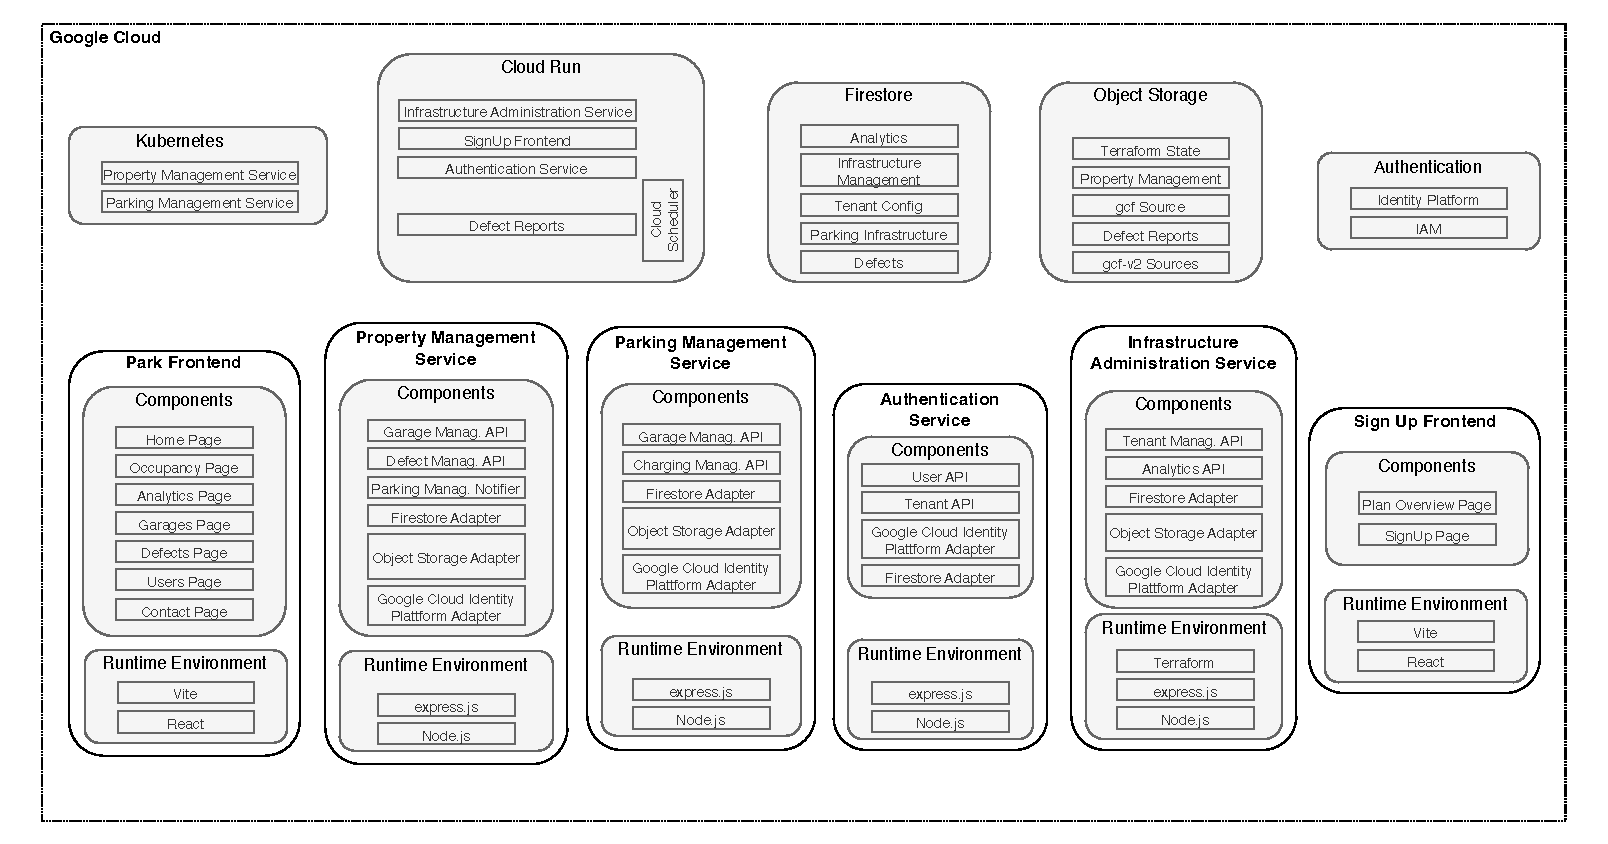
\includegraphics[width=\textwidth]{resources/03-runtime-view/pdf/architecture.pdf}
  \caption{Alle Mircoservices}
  \label{fig:system-architecture}
\end{figure}

In Abbildung \ref{fig:cloud-ressources} ist die Übersicht über die Cloud Ressourcen dargestellt. 
Die Cloud Ressourcen sind in zwei Gruppen unterteilt:
\paragraph{}

\begin{figure}[ht]
  \centering
  \includegraphics[width=\textwidth]{resources/03-runtime-view/pdf/authentication-sequence.pdf}
  \caption{Ablauf der Tenant Typ abhängigen Authentifizierung}
  \label{fig:authentication-sequence}
\end{figure}


\begin{figure}[ht]
  \centering
  \includegraphics[width=0.95\textwidth]{resources/03-runtime-view/pdf/components-frontend-park.pdf}
  \caption{Alle verwendeten Komponenten, wenn ein Client mit dem Park Frontend interagiert, mit Berücksichtigung von Multitenancy}
  \label{fig:03-components-park-frontend}
\end{figure}

\begin{figure}[ht]
  \centering
  \includegraphics[width=\textwidth]{resources/03-runtime-view/pdf/components-frontend-signup.pdf}
  \caption{Alle verwendeten Komponenten, wenn ein Client mit dem Signup Frontend interagiert}
  \label{fig:03-components-signup-frontend}
\end{figure}

\subsection{Mircoservices}
\subsection{Data Stores}
\goodbreak
\section{DevOps}

Im Folgenden werden alle Aspekte des DevOps-Prozesses beschrieben, 
die für die Entwicklung und den Betrieb der Anwendung relevant sind. 
Dies beinhaltet die Bereitstellung von Umgebungen, Rollen und Serviceaccounts, 
Pipelines und die Veröffentlichung neuer Features, die Einrichtung neuer Tenants, 
das Monitoring und das Load Testing.

\subsection{Umgebungen / Environments}

Für die Entwicklung und den Betrieb der Anwendung werden verschiedene Umgebungen (Environments) verwendet.
Für den Betrieb der Anwendung wird die \glqq{}Production\grqq{}-Umgebung verwendet, für 
die Entwicklung wird die \glqq{}Staging\grqq{}-Umgebung verwendet. 
Eine weitere \glqq{}Development\grqq{}-Umgebung wurde aufgrund der geringen Anzahl an Entwicklern 
nicht eingerichtet. Werden für die lokale Entwicklung Cloud-Dienste wie Firestore oder 
Storage Buckets benötigt, werden der Einfachheit halber diese aus der \glqq{}Staging\grqq{}-Umgebung 
verwendet.

Jede Umgebung wird in einem eigenen Projekt in der Google Cloud Platform betrieben.
So wird eine klare Trennung zwischen den Umgebungen gewährleistet.
Da beide Umgebungen über IAC (Infrastructure as Code) verwaltet werden,
sind die Umgebungen identisch und können außerdem schnell wiederhergestellt werden.

\subsubsection{Ressourcen pro Umgebung}

Tabelle \ref{tab:google-cloud-ressourcen} listet die Google Cloud Ressourcen pro Umgebung auf und
beschreibt kurz deren Funktion. Da die Umgebungen identisch sind, ist nur eine Tabelle notwendig.

\renewcommand{\arraystretch}{1.5}
{\rowcolors{2}{}{gray!20}
\begin{longtable}{l p{10cm}}
  \caption{Google Cloud Ressourcen pro Umgebung}
  \label{tab:google-cloud-ressourcen} \\
  \textbf{Ressource} & \textbf{Beschreibung} \\ [1ex]
  Kubernetes Cluster & Cluster, auf dem die Anwendung läuft. \\ [0.5ex]
  Storage Buckets  & Storage Buckets zur Speicherung von Defect Bildern, Defect Reports und anderen Dateien wie z.B. den Terraform State Files. \\ [0.5ex]
  Firestore & Firestore Datenbank zur Speicherung von Daten. \\ [0.5ex]
  Identity Platform & Identity Platform zur Verwaltung von Benutzern und Tenants \\ [0.5ex]
  Identity Federation & Identity Federation zur Authentifizierung von GitHub ohne Credentials. \\ [0.5ex]
  Cloud Run & Cloud Run für Services, die nicht im Kubernetes Cluster laufen. \\ [0.5ex]
  Artifact Registry & Ein Repository für Docker Images in der Artifact Registry \\ [0.5ex]
  DNS Zone & DNS Zone zur Verwaltung der Subdomains der einzelnen Tenants. \\ [0.5ex]
\end{longtable}}

\subsubsection{Tenant Isolation}

Die Isolation der Tenants im Kubernetes Cluster wird durch die Verwendung von Namespaces erreicht.
Es gibt einen Namespace für die \textit{free} Tenants und einen für die \textit{premium} Tenants.
Die Tenants in den \textit{free} bzw. \textit{premium} Namespaces teilen sich die dem Namespace zugewiesenen Ressourcen.
Enterprise Tenants erhalten einen eigenen Namespace. 
Die darin enthaltenen Ressourcen sind nur für diesen Tenant verfügbar.

Die Isolation der Tenants in der Google Cloud Platform wird durch die Verwendung von 
separaten Buckets und Firestore Datenbanken erreicht. Die Ressourcen werden dabei 
analog zu den Kubernetes Namespaces aufgeteilt. Die \textit{free} und \textit{premium} Tenants
teilen sich die Ressourcen wie Buckets und Firestore Datenbanken. Die Enterprise Tenants
erhalten eigene Ressourcen.

Für die Isolation innerhalb der geteilten Ressourcen, werden in den Buckets Unterordner und in 
den Firestore Datenbanken separate Collections für die Tenants angelegt.

\subsection{Roles and Role Mapping}

Da das Team aus nur drei Mitgliedern besteht, wurde auf eine detaillierte Aufteilung der Rollen unter
den Teammitgliedern verzichtet. Jedes Teammitglied hat Zugriff auf alle Ressourcen in dem jeweiligen Projekt.
Dafür wurde jedem Teammitglied die Rolle \textit{roles/owner} zugewiesen.

\subsubsection{Dienstkonten}

Um die einzelnen Services der Park Anwendung zu authentifizieren, wurde pro Service ein Dienstkonto erstellt.
Genauer wurde pro Service pro Namespace ein Dienstkonto angelegt weil ein Service aus dem \textit{free}
Namespace nicht auf die Ressourcen eines Services aus dem \textit{premium} Namespace zugreifen darf.

Um keine Credentials in den Services speichern zu müssen, 
wurde die \glqq{}Workload Identity Federation for GKE\grqq{}\footnote{https://cloud.google.com/kubernetes-engine/docs/concepts/workload-identity} verwendet.
Diese muss bei der Erstellung des Clusters aktiviert werden und läuft auf den Nodes des Clusters. 
Die Workload Identity Federation unterscheidet zwischen Dienstkonten 
der Google Cloud Platform und Dienstkonten des Kubernetes Clusters.

\begin{itemize}
  \item \textbf{Kubernetes-Dienstkonten} sind Kubernetes-Ressourcen, die eine Identität für Prozesse bereitstellen, 
  die in Ihren GKE-Pods ausgeführt werden.
  \item \textbf{IAM-Dienstkonten} sind Google Cloud-Ressourcen, 
  mit denen Anwendungen autorisierte Aufrufe an Google Cloud APIs ausführen können.
\end{itemize}

Die Workload Identity Federation ermöglicht es, dass ein Kubernetes-Dienstkonto auf ein IAM-Dienstkonto gemappt wird.
Damit das Mapping funktioniert, muss das Kubernetes-Dienstkonto in der Annotation 
\textit{iam.gke.io/gcp-service-account} die E-Mail-Adresse des IAM-Dienstkontos enthalten.
\footnote{https://cloud.google.com/kubernetes-engine/docs/how-to/workload-identity\#kubernetes-sa-to-iam}


Um den Zugriff auf die Google Cloud Ressourcen aus GitHub Actions zu ermöglichen,
wurde pro Projekt ein weiteres Dienstkonto erstellt. Dieses Dienstkonto hat nur die minimalen Rechte,
die für die Ausführung der GitHub Actions notwendig sind. Durch die \glqq{}Workload Identity Federation\grqq{}
(das ist eine andere Workload Identity Federation als die für GKE) müssen keine Credentials
in den GitHub Secrets gespeichert werden.\footnote{https://cloud.google.com/blog/products/identity-security/enabling-keyless-authentication-from-github-actions?hl=en}

\subsection{Pipelines and Release of new Features}

Für die Bereitstellung von neuen Features und Bugfixes wird ein CI/CD-Prozess verwendet.
Die CI/CD-Pipeline wird mit GitHub Actions realisiert.
Die gesamte Pipeline ist in mehrere Actions unterteilt, wobei die eine Action bei Pull-Requests ausgeführt wird,
die andere bei einem Push auf den \textit{dev}- oder \textit{main}-Branch.

\subsubsection*{Pipeline für Pull-Requests auf \textit{dev} und \textit{main}}

Die Pipeline für Pull-Requests besteht aus den folgenden Jobs:
\begin{itemize}
  \item \textbf{Build}: Die Docker Images aller Services werden gebaut und auf eventuelle Fehler überprüft.
  \item \textbf{Test}: Die Unittests der Services werden ausgeführt.
  \item \textbf{Plan Terraform for the Infrastructure}: Die Änderungen an der Infrastruktur werden geplant.
  \item \textbf{Plan Terraform for the Application}: Die Änderungen an der Anwendung werden geplant.
\end{itemize}

Je nachdem, ob es sich um einen Push auf den \textit{dev}- oder \textit{main}-Branch handelt, wird die Pipeline
für die \textit{staging}- oder \textit{production}-Umgebung ausgeführt. 
Abbildung \ref{fig:pr-pipeline} zeigt die Pipeline für Pull-Requests.

\begin{figure}[H]
  \centering
  \includegraphics[width=0.6\textwidth]{resources/pr-pipeline.pdf}
  \caption{PR Pipeline}
  \label{fig:pr-pipeline}
\end{figure}


\subsubsection*{Pipeline für Push auf \textit{dev} und \textit{main}}

Die Pipeline für einen Push auf den \textit{dev}- oder \textit{main}-Branch ist für das 
Deployment der Änderungen in der Infrastruktur und der Anwendung zuständig.
Die Pipeline besteht aus den folgenden Jobs:

\begin{itemize}
  \item \textbf{Apply Terraform for the Infrastructure}: Die Änderungen an der Infrastruktur werden angewendet.
  \item \textbf{Build and Push Images}: Die Docker Images aller Services werden gebaut und in die Artifact Registry hochgeladen.
  \item \textbf{Package Cloud Functions}: Die Cloud-Functions werden in ein Zip-Archiv gepackt.
  \item \textbf{Apply Terraform for the Application}: Die Änderungen an der Anwendung werden angewendet. Das beinhaltet das Deployment der Docker Images und der Cloud-Functions.
  \item \textbf{Deploy Cloud Run}: Cloud-Run-Services, die nicht im Kubernetes Cluster laufen, werden deployed.
  \item \textbf{Update deployment.json}: Deployment-Informationen wie der Tag der Images werden in einer JSON-Datei in einem Bucket für spätere Pipelines gespeichert.
\end{itemize}

Da die Park Anwendung Multi-Tenant-fähig ist, müssen die Tenants auch in den Pipelines berücksichtigt werden.
Viele Ressourcen wie Buckets, Firestore Datenbanken und DNS-Zonen müssen pro Enterprise Tenant erstellt werden.
Um herauszufinden, ob Ressourcen erstellt, aktualisiert oder gelöscht werden müssen, wird eine JSON-Datei 
aus einem Bucket geladen. Diese Datei enthält die Konfiguration der Enterprise Tenants.

Je nachdem, ob es sich um einen Push auf den \textit{dev}- oder \textit{main}-Branch handelt, wird die Pipeline
für die \textit{staging}- oder \textit{production}-Umgebung ausgeführt.
Abbildung \ref{fig:cd-pipeline} zeigt die Pipeline für einen Push auf den \textit{dev}- oder \textit{main}-Branch.

\begin{figure}[H]
  \centering
  \includegraphics[width=\textwidth]{resources/cd-pipeline.pdf}
  \caption{CD Pipeline}
  \label{fig:cd-pipeline}
\end{figure}


\subsection{New Tenants}

Wenn ein neuer Client die Park Anwendung verwenden möchte und über das Sign-Up-Frontend(\ref{sec:signup-frontend})
das Anmeldeformular ausgefüllt hat, wird ein Request an den Authentication Service(\ref{sec:auth-service}) gesendet.
Der Authentication Service erstellt einen neuen Tenant in der Identity Platform und in der Firestore Datenbank.
Neben dem Tenant wird auch ein Admin-Benutzer für den neuen Tenant erstellt. Der Admin-Benutzer 
erhält die vom Client angegebene E-Mail-Adresse und das vom Client angegebene Passwort.

Anschließend wird ein Request an den Infrastructure Service gesendet.
Handelt es sich um einen \textit{free} oder \textit{premium} werden keine Änderungen an der Infrastruktur vorgenommen.
Handelt es sich um einen Enterprise Tenant, wird ein Request an GitHub gesendet, der
den Workflow für die Erstellung der Ressourcen für den neuen Tenant startet.

\subsubsection{Erstellung der Ressourcen für Enterprise Tenants}

Die Erstellung der Ressourcen für Enterprise Tenants erfolgt über einen GitHub Workflow.
Der Workflow bekommt als Input die Tenant-ID und die Subdomain des Tenants.
Der im Folgenden etwas genauer beschriebene Workflow ist in Abbildung \ref{fig:tenant-pipeline} dargestellt.
Der Workflow besteht aus den folgenden Jobs:
\begin{itemize}
  \item \textbf{Manage enterprise tenants}: Der Workflow fügt die neue Konfiguration des Enterprise Tenants zur JSON-Datei hinzu.
  \item \textbf{Load deployment.json}: Die JSON-Datei mit den Informationen über das aktuelle Deployment wird geladen. Hier wird der
  Tag der Docker Images ausgelesen. Weil die aktuell deployten Services nicht verändert werden sollen, sondern nur neue Services 
  hinzugefügt werden sollen, wird der Tag der Images benötigt.
  \item \textbf{Load enterprise-tenants.json}: Die im vorherigen Schritt aktualisierte JSON-Datei wird geladen. Der Inhalt der JSON-Datei
  wird in einer Umgebungsvariable gespeichert, damit die folgenden Jobs darauf zugreifen können.
  \item \textbf{Apply Terraform for the Application}: Mithilfe von Terraform werden \textbf{alle} Ressourcen für den neuen Tenant erstellt.
\end{itemize}

\begin{figure}[H]
  \centering
  \includegraphics[width=\textwidth]{resources/tenant-pipeline.pdf}
  \caption{Tenant Pipeline}
  \label{fig:tenant-pipeline}
\end{figure}

\subsection{Monitoring}

Für das Monitoring der Anwendung wird Google Cloud Monitoring verwendet.
Einerseits bietet Google Cloud Monitoring eine Vielzahl von Metriken und vorkonfigurierte Dashboards,
andererseits können auch eigene Dashboards erstellt werden.

Für die Überwachung der Anwendung und der durch die Tenants verursachten Last werden 
vor allem folgende Metriken überwacht:

\begin{itemize}
  \item \textbf{CPU Utilization}: Überwachung der CPU-Auslastung pro Namespace.
  \item \textbf{Memory Utilization}: Überwachung des Speicherverbrauchs pro Namespace.
  \item \textbf{Request Count}: Überwachung der Anzahl der Requests pro Namespace.
\end{itemize}

Abbildung \ref{fig:monitoring-dashboard} zeigt eines der Dashboards zum Monitoring der Park Anwendung.

\begin{figure}[H]
  \centering
  \includegraphics[width=\textwidth]{resources/Monitoring.png}
  \caption{Monitoring Dashboard}
  \label{fig:monitoring-dashboard}
\end{figure}

\subsection{Load Testing}

Für das Load Testing wurde Grafana k6\footnote{\url{https://k6.io/}} verwendet. K6 ist ein Open-Source-Tool,
das für das Load Testing von APIs und Webseiten verwendet werden kann.

Um zu zeigen, dass die Park Anwendung bei steigender Last die Microservices skalieren kann und bei hoher 
Last stabil bleibt, wurde ein Load Test durchgeführt, der die Anwendung mit 2000 Benutzern für 20 Minuten belastet.
Der Load Test wurde auf die \textit{staging}-Umgebung durchgeführt. 

Um die Wirkung des Horizontal Pod Autoscalers (HPA) und den Ressource Quotas zu zeigen, wurden die Quotas so gesetzt,
dass die der HPA die Anzahl der Pods auf maximal 9 erhöhen kann, bevor die Quotas erreicht werden. Außerdem wurde mit 
dem Load Test überprüft, ob sich die Namespaces gegenseitig beeinflussen oder ob die Quotas das Noisy Neighbor Problem verhindern.

Der Load Test führt folgende drei Schritte aus:
\begin{enumerate}
  \item In eine Garage einfahren und ein Ticket ziehen.
  \item Das Ticket bezahlen.
  \item Die Garage verlassen.
\end{enumerate}

Da es sich bei diesen drei Schritten um die häufigsten Aktionen handelt, die ein Benutzer in der Park Anwendung durchführt,
wurden diese für den Load Test ausgewählt. Der Code für den Load Test ist im Anhang \ref{app:load-test-code} zu finden.

Abbildung \ref{fig:load-testing} zeigt wie die Anwendung auf die steigende Last reagiert und wie die Pods skaliert werden.
Das untere Diagramm in Abbildung \ref{fig:load-testing} zeigt die Anzahl der Pods des Parking Management Services pro Namespace.
Die Anzahl der angeforderten Pods steigt im free und im enterprise Namespace auf 10 an, die Anzahl der verfügbaren 
Pods erreicht jedoch jeweils nur 9. Das liegt daran, dass die Quotas so gesetzt sind, dass der HPA maximal 9 Pods 
erstellen kann. Der HPA hat also die Pods erfolgreich skaliert, bis die Quotas erreicht wurden.

\begin{figure}[H]
  \centering
  \includegraphics[width=\textwidth]{resources/LoadTest.png}
  \caption{Load Testing}
  \label{fig:load-testing}
\end{figure}

Die Werte der Quotas und der HPAs sind Werte, die für die Demonstration der Skalierung gewählt wurden und nicht über längere Zeit getestet wurden.
In einer produktiven Umgebung sollte die Anwendung über längere Zeit getestet werden, um die optimalen Werte für die Quotas und HPAs zu finden. 
\goodbreak
\section{Commercial Model}
\subsection{Tenant Types}

\paragraph{Free Tenant}
Der Free-Plan richtet sich an Nutzer, die grundlegende Funktionen zur Verwaltung von Standorten und Infrastruktur benötigen. Die zentralen Merkmale dieses Plans sind:
\begin{itemize}
	\item \textbf{Parkhausverwaltung:} Erstellung und Verwaltung mehrerer Parkhäuser zur effizienten Organisation von Standorten.
	\item \textbf{Defektmanagement:} Nachverfolgung und Bearbeitung von Defekten zur schnellen Problemlösung.
	\item \textbf{Integration von E-Mobility-Ladestationen:} Einbindung und Überwachung der Ladeinfrastruktur für Elektrofahrzeuge.
\end{itemize}
Der Free-Plan stellt essenzielle Werkzeuge zur Verwaltung von Parkhäusern und Ladestationen bereit, ohne monatliche Kosten zu verursachen.

\paragraph{Premium Tenant}
Der Premium-Plan bietet die gleiche Grundfunktionalität wie der Free-Plan, richtet sich jedoch an Organisationen mit höheren Anforderungen an Benutzerverwaltung, Analysen und Systemleistung.
Zu den Funktionen gehören:
\begin{itemize}
	\item \textbf{Benutzerverwaltung:} Unbegrenzte Benutzeranzahl mit erweiterten Zugriffskontrollen.
	\item \textbf{E-Mobility-Ladestationen:} Erweiterte Integration und Verwaltung von Ladeinfrastrukturen.
	\item \textbf{Mehrsprachigkeit:} Unterstützung mehrerer Sprachen für internationale Nutzung.
	\item \textbf{Analytik-Dashboard:} Bereitstellung detaillierter Analysen zur Prozessoptimierung.
	\item \textbf{Optimierte Performance:} Schnellere Ladezeiten und höhere Systemzuverlässigkeit.
	\item \textbf{Premium-Support:} Priorisierte Kundenbetreuung für effiziente Problemlösungen.
	\item \textbf{Erhöhte Sicherheit:} Erweiterte Sicherheitsfunktionen zum Schutz sensibler Daten.
\end{itemize}
\textbf{Kosten:}
\begin{itemize}
	\item \textbf{79,90 €/Monat} Grundgebühr.
	\item \textbf{1 €/Benutzer.}
	\item \textbf{5 €/10.000 Backend-Requests.}
\end{itemize}

\paragraph{Enterprise Tenant}
Der Enterprise-Plan umfasst die Funktionen des Premium-Plans und ist für große Organisationen konzipiert, die maximale Leistung, Sicherheit und Support benötigen.
Er beinhaltet:
\begin{itemize}
	\item \textbf{Anpassbarkeit:} Bereitstellung einer dedizierten Domain.
	\item \textbf{Maximale Performance:} Höchste Geschwindigkeit und Systemstabilität.
	\item \textbf{Priorisierter Support:} Bevorzugte Bearbeitung aller Anfragen.
	\item \textbf{Erweiterte Sicherheitsstandards:} Umfassender Schutz sensibler Daten.
\end{itemize}
\textbf{Kosten:}
\begin{itemize}
	\item \textbf{129,90 €/Monat} Grundgebühr.
	\item \textbf{5 €/10.000 Backend-Requests.}
\end{itemize}

\subsection{Pricing Model}
Das Preismodell der Plattform bietet flexible Tarife, die auf verschiedene Nutzeranforderungen zugeschnitten sind.
Die Preisstruktur ermöglicht eine skalierbare Nutzung entsprechend der Anzahl der Benutzer und Backend-Anfragen.

\begin{table}[h!]
	\centering
	\caption{Preisübersicht der Tenant-Typen}
	{\rowcolors{2}{}{gray!20}
		\begin{tabularx}{\textwidth}{|l|X|X|X|}
			\hline
			\textbf{Plan} & \textbf{Grundgebühr (€/Monat)} & \textbf{Preis pro Benutzer (€/Monat)} & \textbf{Preis pro 10.000 Backend-Requests (€/Monat)} \\ \hline
			Free          & 0,00                           & -                                     & -                                                    \\ \hline
			Premium       & 79,90                          & 1,00                                  & 5,00                                                 \\ \hline
			Enterprise    & 129,90                         & -                                     & 5,00                                                 \\ \hline
		\end{tabularx}}
	\label{tab:pricing}
\end{table}

Diese Preisgestaltung ermöglicht sowohl kleinen als auch großen Organisationen eine anpassbare und kosteneffiziente Nutzung der Plattform.

\subsection{Cost Model}
Das Kostenmodell basiert auf einer optimierten Ressourcennutzung und unterscheidet sich je nach Tenant-Typ:
\begin{itemize}
	\item \textbf{Free-Plan:} Mandanten teilen sich einen Kubernetes-Namespace, eine gemeinsame Firestore-Datenbank und gemeinsamen Cloud-Storage.
	\item \textbf{Premium-Plan:} Gemeinsame Nutzung eines Kubernetes-Namespaces mit erhöhter Ressourcenallokation, gemeinsamer Firestore-Datenbank und Cloud-Storage.
	\item \textbf{Enterprise-Plan:} Dedizierte Kubernetes-Namespaces, eigene Firestore-Datenbank und eigener Cloud-Storage pro Mandant.
	\item \textbf{Geteilte Services:} Drei zentrale Cloud-Run-Services werden von allen Mandanten genutzt.
\end{itemize}

Für unsere Kalkulation haben wir den Google Cloud Pricing Calculator verwendet, um die Kosten für die verschiedenen Ressourcen zu schätzen. Hier der Link zu unserer Konfiguration \href{https://cloud.google.com/products/calculator?hl=de&dl=CjhDaVExWXpBNE5UUm1OaTA0TUdKaUxUUTFPVFl0T0dGa09DMWxZVEEzTVdZeVlXSm1ZalVRQVE9PRAJGiQzREI3QkJCQS04Nzc0LTQ5RTEtODY5Qy1DQjVCREI5NzlGMDM}{Calculator}. Hier sind jedoch nur die Kosten für eine Umgebung zu sehen, da wir eine identische Production und Staging Umgebung haben, verdoppeln sich die Kosten.  \\

\begin{table}[h!]
	\centering
	\caption{Ressourcennutzung und monatliche Kostenschätzung}
	{\rowcolors{2}{}{gray!20}
		\begin{tabularx}{\textwidth}{|l|X|X|X|}
			\hline
			\textbf{Ressource}    & \textbf{Free-Plan}              & \textbf{Premium-Plan} & \textbf{Enterprise-Plan (pro Mandant)} \\ \hline
			Kubernetes Namespace  & 135 €/Monat                     & 135 €/Monat           & 400 €/Monat (gesamt) = 40 €/Monat (pro Tenant)                          \\ \hline
			Firestore-Datenbank   & 2 €/Monat                       & 2 €/Monat             & 2 €/Monat                              \\ \hline
			Cloud Storage         & 4 €/Monat                       & 4 €/Monat             & 4 €/Monat                              \\ \hline
			Cloud Functions       & 6 €/Monat                       & 6 €/Monat             & 6 €/Monat                              \\ \hline
			Geteilte Services     & \multicolumn{3}{c|}{60 €/Monat}                                                                  \\ \hline
			\textbf{Gesamtkosten} & 167 €/Monat                     & 167 €/Monat           & $\sim 54$ €/Monat                      \\ \hline
		\end{tabularx}}
	\label{tab:costmodel}
\end{table}

In Tabelle \ref{tab:costmodel} werden die geschätzten Kosten für die verschiedenen Pläne dargestellt.
Diese Kosten sind auf Staging und Production Umgebung zusammen berechnet.
Dabei wurden die Enterprise Namespace Kosten durch zehn geteilt (Annahme wir haben 10 Enterprise Kunden) und die der Geteilte Services Anteil von 20€ auch nochmal , um die Verteilung der Ausgaben für einzelne Mandanten zu berücksichtigen.
Unter geteilten Kosten sind die Kosten für die drei Services (Authentication Service mit Datenbank, Infrastructure Management Service mit Datenbank und Sign Up Frontend), die von allen Mandanten gemeinsam genutzt werden, zusammengefasst.
\\
Die wichtigsten Punkte sind:
\begin{itemize}
	\item \textbf{Free Plan:} Die Gesamtkosten belaufen sich auf geschätzte 167 €/Monat durch die gemeinsame Nutzung von Ressourcen.
	\item \textbf{Premium Plan:} Die Gesamtkosten belaufen sich auf geschätzte 167 €/Monat durch die gemeinsame Nutzung von Ressourcen.
	\item \textbf{Enterprise Plan:} Jeder Enterprise-Mandant verursacht individuelle Kosten von rund 54 €/Monat. Dies ist bedingt durch die exklusive Zuweisung von Ressourcen wie Kubernetes-Namespace, Firestore-Datenbank und Cloud Storage.
\end{itemize}

Dieses Kostenmodell bietet eine klare Grundlage für die wirtschaftliche Planung und Skalierung der Plattform.

\paragraph{Worst-Case-Szenario}
Wir haben nur Free Kunden, die alle die maximale Anzahl an Backend-Requests verursachen und keine Premium und Enterprise Kunden.
Das heißt wir Kubernetes Cluster läuft ohne dass die Ressourcen genutzt werden und die geteilten Services bleiben auch gleich teuer.
Dann fallen folgende Kosten an:
\begin{itemize}
	\item \textbf{Kubernetes Namespace:} 135 (free) + 135 (premium) + 400 (enterprise) = 670 €/Monat
	\item \textbf{Firestore-Datenbank:} 2 €/Monat
	\item \textbf{Cloud Storage:} 4 €/Monat
	\item \textbf{Cloud Functions:} 6 €/Monat
	\item \textbf{Geteilte Services:} 60 €/Monat
	\item \textbf{Gesamtkosten:} 742 €/Monat
\end{itemize}
Das heißt wir würden im Worst Case Szenario 742 €/Monat minus machen.

\paragraph{Realitisches Szenario}
Über 10 Enterprise Kunden, die alle auch die maximale Anzahl an Backend-Requests verursachen (10.000 für einfachere Rechnung) und über 10 Premium Kunden die auch ebenfalls die maximale Backend-Requests (10.000 für einfachere Rechnung) erreichen und zusammen 40 Nutzer haben.
Free Kunden und Premium Kunden sind irrelevant da sie monatlich immer die gleichen Fixkosten verursachen.
Dann fallen folgende Kosten an:
\begin{itemize}
	\item \textbf{Kubernetes Namespace:} 135 (free) + 135 (premium) + 400 (enterprise) = 670 €
	\item \textbf{Firestore:} 2 (free) + 2 (premium) + 20 (enterprise) = 24 €
	\item \textbf{Cloud Storage:} 4 (free) + 4 (premium) + 40 (enterprise) = 48 €
	\item \textbf{Cloud Functions:} 6 (free) + 6 (premium) + 60 (enterprise) = 72 €
	\item \textbf{Geteilte Services:} 60 €
	\item \textbf{Gesamtkosten:} 874 €/Monat
\end{itemize}
Das heißt wir würden im Realistischen Szenario 874 €/Monat an Kosten zahlen.
Jedoch folgende Einnahmen generieren:
\begin{itemize}
	\item \textbf{Enterprise Kunden:} 10 * 129,90 € = 1299 €
	\item \textbf{Premium Kunden:} 10 * 79,90 € = 799 €
	\item \textbf{Benutzer:} 40 * 1,00 € = 40 €
	\item \textbf{Backend-Requests:} 20 * 5,00 € = 50 €
	\item \textbf{Gesamteinnahmen:} 2238 €
\end{itemize}

Das heißt wir würden im Realistischen Szenario (Annahme nur 10 Enterprise und 10 Premium Tenants ist eher pessimistisch) 1364 €/Monat an Gewinn machen.

\paragraph{Best-Case-Szenario}
Das Best-Case-Szenario wäre, wenn wir sehr viele Enterprise Kunden haben, die alle weit über 10.000 Backend-Requests senden und viele Premium Kunden, die viele Nutzer erstellt haben und monatlich viele (über 10.000 pro Tenant) Backend-Requests senden.
Die Free Kunden sind irrelevant da sie monatlich immer die gleichen Fixkosten verursachen und uns keinen Gewinn einbringen.

\goodbreak

\goodbreak

\end{sloppypar}
\end{document}
